\normaltrue \difficilefalse \tdifficilefalse
\correctionfalse
%\UPSTIidClasse{11} % 11 sup, 12 spé
%\newcommand{\UPSTIidClasse}{11}

\exer{ $\star$ \label{C2:03:stab:64}}
%% CCP MP 2007
\setcounter{numques}{0}
\UPSTIcompetence[2]{C2-03}
\index{Compétence C2-03}
\index{Schéma-blocs}
\index{Stabilite}

\ifcorrection
\else
\textbf{Pas de corrigé pour cet exercice.}
\fi

L'asservissement est donné par le schéma-blocs suivant. $H_{\text{BO}}(p) = \dfrac{4}{p\left( p+3,6\right)}$.  Le retard du système est de \SI{0,2}{s}.
De plus, $C(p)=K_c\dfrac{1+T_c p}{T_c p}$

\begin{center}
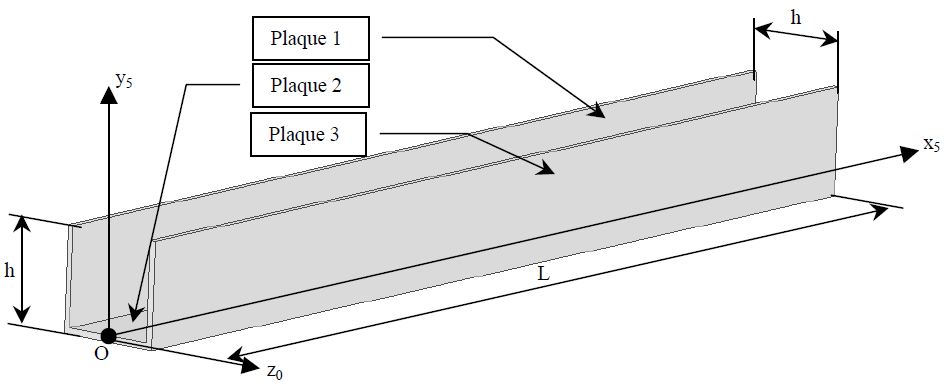
\includegraphics[width=\linewidth]{64_01}
\end{center}

 
\question{Tracer le diagramme de Bode asymptotique de $H_{\text{BO}}(p)$ pour des pulsations comprises entre \SI{0,5}{rad.s^{-1}} et \SI{50}{rad.s^{-1}}.}
\ifprof
\else 
\fi

\question{Tracer le diagramme de Bode du retard pour des pulsations comprises entre \SI{0,5}{rad.s^{-1}} et \SI{50}{rad.s^{-1}}.}
\ifprof
\else 
\fi


On donne le diagramme de la FTBO retardée. 

\begin{center}
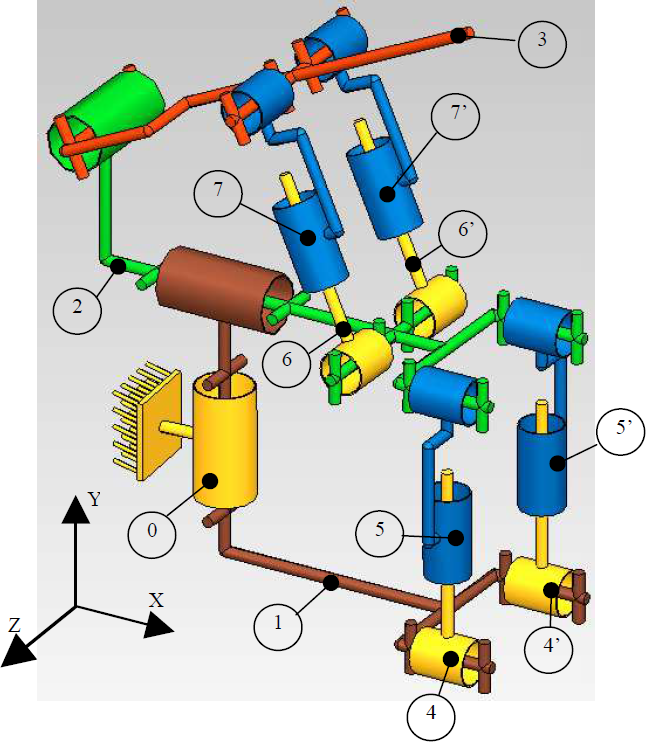
\includegraphics[width=\linewidth]{64_02}
\end{center}

\question{Déterminer le gain $K_c$ qui donne une marge de phase de 50\degres.}
\ifprof
\else 
\fi

\question{La constante $T_c$ qui laisse subsister une marge de phase d’environ 45\degres.}
\ifprof
\else 
\fi


\question{Quelle est l’erreur de traînage du système corrigé pour l’entrée en rampe
considérée (en négligeant le retard).}
\ifprof
\else 
\fi


\ifprof
\else

\noindent\footnotesize
% \fbox{\parbox{.9\linewidth}{
% Éléments de corrigé : 
% \begin{enumerate}
  % \item $\varepsilon_{\text{con \%}} = \dfrac{1}{1+K_PK_m K_{\text{pom}} K_{\text{cap}} }$;
  % \item $K_P > 19$;
  % \item $\varepsilon_{\text{pert}} = \Delta Q_e \dfrac{K_f}{1+K_{\text{cap}}K_PK_mK_{\text{pom}}}$;
  % \item $K_P > 2,19$.
  % \item $K_P < 0,125$. Il est impossible de vérifier les trois conditions avec un correcteur proportionnel.
% \end{enumerate}}}
\normalsize

\begin{flushright}
\footnotesize{Corrigé  voir \ref{C2:03:stab:64}.}
\end{flushright}%
\fi